%%%%%%%%%%%%%%%%%%%%%%%%%%%%%%%%%%%%%%%%%
% Beamer Presentation
% LaTeX Template
% Version 1.0 (10/11/12)
%
% This template has been downloaded from:
% http://www.LaTeXTemplates.com
%
% License:
% CC BY-NC-SA 3.0 (http://creativecommons.org/licenses/by-nc-sa/3.0/)
%
%%%%%%%%%%%%%%%%%%%%%%%%%%%%%%%%%%%%%%%%%

%----------------------------------------------------------------------------------------
%	PACKAGES AND THEMES
%----------------------------------------------------------------------------------------

\documentclass[UTF8,aspectratio=169,12pt]{ctexbeamer}

\usepackage{hyperref}
\hypersetup{
	colorlinks=true,
	linkcolor=red,
	anchorcolor=blue,
	citecolor=green
}

\mode<presentation> {
	
	% The Beamer class comes with a number of default slide themes
	% which change the colors and layouts of slides. Below this is a list
	% of all the themes, uncomment each in turn to see what they look like.
	
	%\usetheme{default}
	%\usetheme{AnnArbor}
	%\usetheme{Antibes}
	%\usetheme{Bergen}
	%\usetheme{Berkeley}
	%\usetheme{Berlin}
	%\usetheme{Boadilla}
	%\usetheme{CambridgeUS}
	%\usetheme{Copenhagen}
	%\usetheme{Darmstadt}
	%\usetheme{Dresden}
	%\usetheme{Frankfurt}
	%\usetheme{Goettingen}
	%\usetheme{Hannover}
	%\usetheme{Ilmenau}
	%\usetheme{JuanLesPins}
	%\usetheme{Luebeck}
	\usetheme{Madrid}
	%\usetheme{Malmoe}
	%\usetheme{Marburg}
	%\usetheme{Montpellier}
	%\usetheme{PaloAlto}
	%\usetheme{Pittsburgh}
	%\usetheme{Rochester}
	%\usetheme{Singapore}
	%\usetheme{Szeged}
	%\usetheme{Warsaw}
	
	% As well as themes, the Beamer class has a number of color themes
	% for any slide theme. Uncomment each of these in turn to see how it
	% changes the colors of your current slide theme.
	
	%\usecolortheme{albatross}
	%\usecolortheme{beaver}
	%\usecolortheme{beetle}
	%\usecolortheme{crane}
	%\usecolortheme{dolphin}
	%\usecolortheme{dove}
	%\usecolortheme{fly}
	%\usecolortheme{lily}
	%\usecolortheme{orchid}
	%\usecolortheme{rose}
	%\usecolortheme{seagull}
	%\usecolortheme{seahorse}
	%\usecolortheme{whale}
	%\usecolortheme{wolverine}
	
	%\setbeamertemplate{footline} % To remove the footer line in all slides uncomment this line
	%\setbeamertemplate{footline}[page number] % To replace the footer line in all slides with a simple slide count uncomment this line
	
	%\setbeamertemplate{navigation symbols}{} % To remove the navigation symbols from the bottom of all slides uncomment this line
}

\usepackage{graphicx} % Allows including images
\graphicspath{{./figs/}}
\usepackage{booktabs} % Allows the use of \toprule, \midrule and \bottomrule in tables
\usepackage{longtable}
\usepackage{xcolor}
\usepackage{minted}
\usepackage{listings}
\lstset{numbers=left, %设置行号位置
	numberstyle=\tiny, %设置行号大小
	keywordstyle=\color{blue}, %设置关键字颜色
	commentstyle=\color[cmyk]{1,0,1,0}, %设置注释颜色
	frame=single, %设置边框格式
	escapeinside=``, %逃逸字符(1左面的键),用于显示中文
	%breaklines, %自动折行
	extendedchars=false, %解决代码跨页时,章节标题,页眉等汉字不显示的问题
	xleftmargin=2em,xrightmargin=2em, aboveskip=1em, %设置边距
	tabsize=4, %设置tab空格数
	showspaces=false %不显示空格
}
% Fonts
% \usepackage{libertine}
% \setmonofont{Courier}
%\setCJKsansfont[ItalicFont=Noto Serif CJK SC Black, BoldFont=Noto Sans CJK SC Black]{Noto Sans CJK SC}


%----------------------------------------------------------------------------------------
% TITLE PAGE
%----------------------------------------------------------------------------------------

\title[第17讲]{第十七讲 :文件系统} % The short title appears at the bottom of every slide, the full title is only on the title page
\subtitle{第4节:虚拟文件系统VFS}
\author{向勇、陈渝、李国良} % Your name
\institute[清华大学] % Your institution as it will appear on the bottom of every slide, may be shorthand to save space
{
  清华大学计算机系 \\ % Your institution for the title page
  \medskip
  \textit{xyong,yuchen,liguoliang@tsinghua.edu.cn} % Your email address
}
\date{\today} % Date, can be changed to a custom date

\begin{document}

\begin{frame}
\titlepage % Print the title page as the first slide
\end{frame}
\section{第4节:虚拟文件系统VFS}
% ## 第十七讲 文件系统
% 
% ### 17.4 VFS
% 
% VFS(共享,缓存):
% 
% \href{https://www.cs.uni.edu/~diesburg/courses/dd/notes/VFS.pptx}{The virtual file system (VFS)}:这里是一个55页的幻灯片,主要介绍VFS的接口;
% 
% \href{https://www.cs.unc.edu/~porter/courses/cse506/s16/slides/vfs.pdf}{Virtual File System}:这也是一个关于VFS的课程幻灯片;
% 
%----------------------------------------------
\begin{frame}
\frametitle{提纲} % Table of contents slide, comment this block out to remove it
\tableofcontents % Throughout your presentation, if you choose to use \section{} and \subsection{} commands, these will automatically be printed on this slide as an overview of your presentation
\end{frame}
%------------------------------------------------
\subsection{Overview}

% 
%------------------------------------------------
\begin{frame}[fragile]
    \frametitle{What is VFS?}

% 
  \begin{figure}
    \centering
    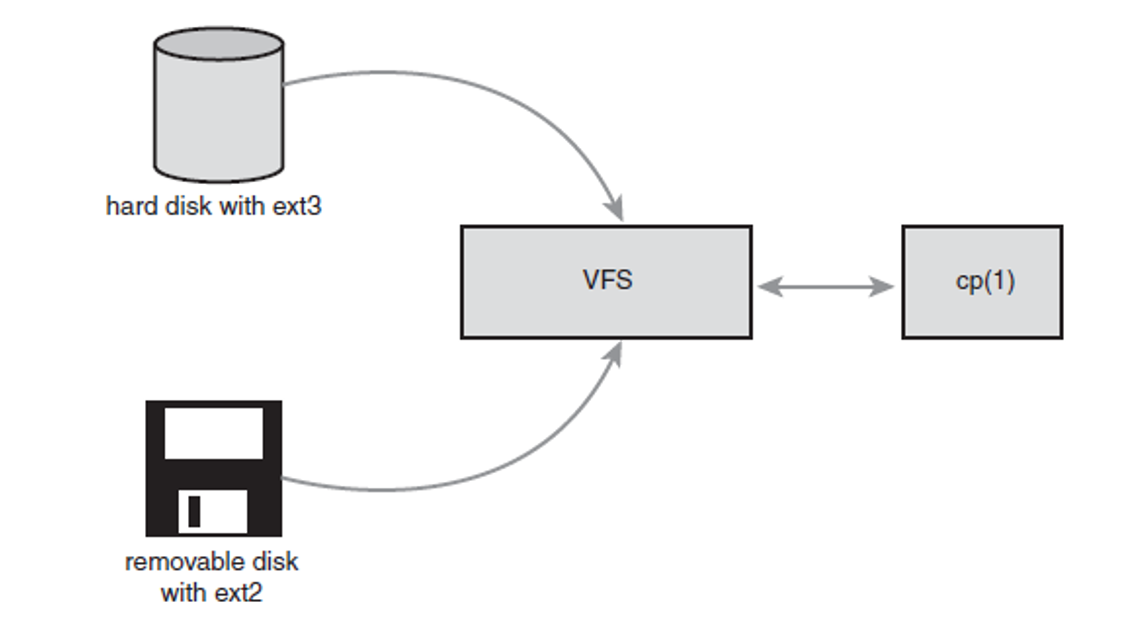
\includegraphics[width=0.5\linewidth]{figs/vfs-example.png}
%		\caption{vfs-example}
	\end{figure}

	    \begin{itemize}
	        \item Common File System Interface
	        \item Basic File Model of File System
	    \end{itemize}
% 
\end{frame}
%------------------------------------------------
\begin{frame}[fragile]
    \frametitle{Common File System Interface}

% 
  \begin{figure}
    \centering
    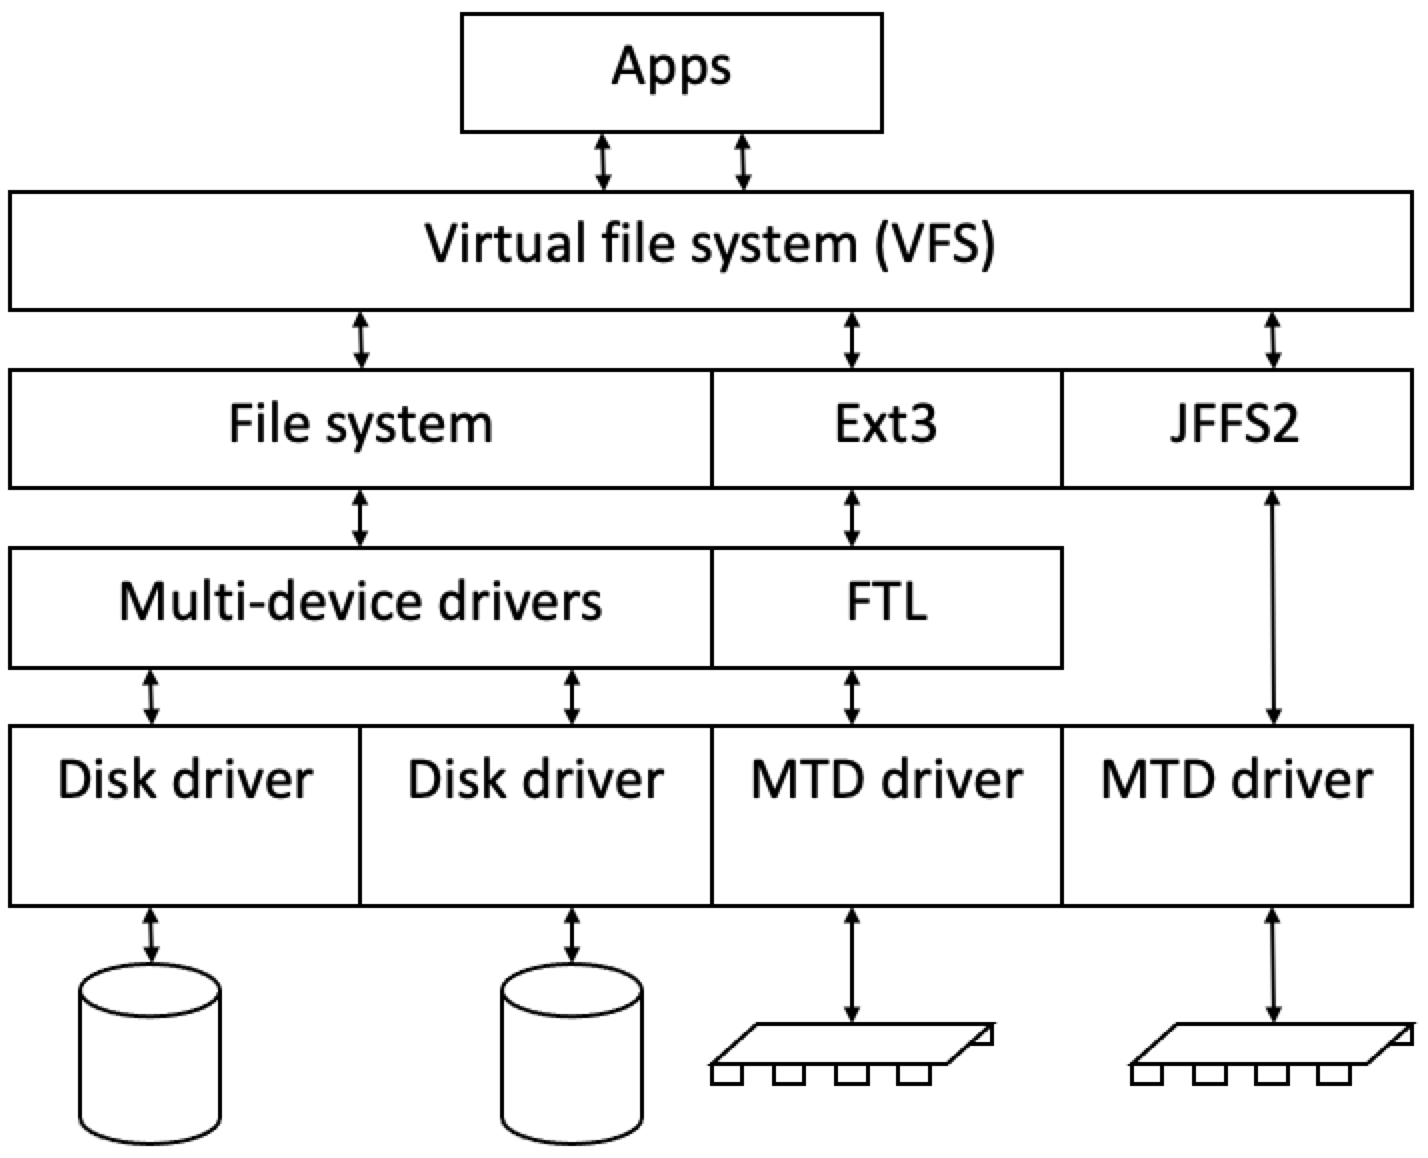
\includegraphics[width=0.4\linewidth]{figs/vfs-interface.png}
%		\caption{vfs-interface}
	\end{figure}


% 
Enables system calls such as open(), read(), and write() to work regardless of file system or storage media
% 
\end{frame}
%------------------------------------------------
\begin{frame}[fragile]
    \frametitle{Basic File Model of File System}

% 
  \begin{figure}
    \centering
    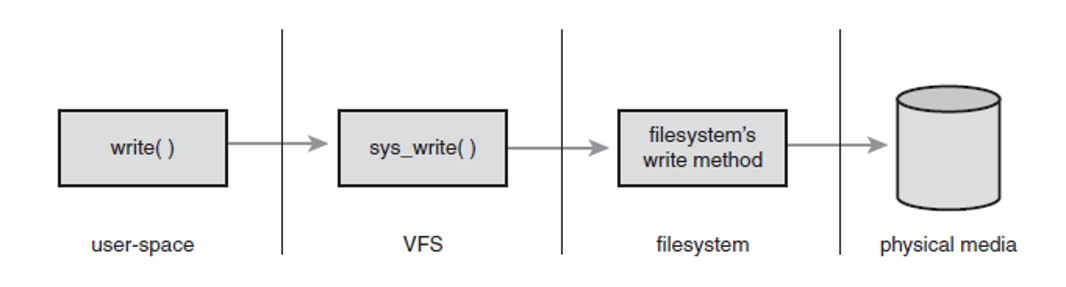
\includegraphics[width=0.8\linewidth]{figs/vfs-Basic-File-Model.png}
		%\caption{vfs-Basic-File-Model}
	\end{figure}



    \begin{itemize}
        \item Defines basic file model conceptual interfaces and data structures
        \item Low level file system drivers actually implement file-system-specific behavior
    \end{itemize}
% 
\end{frame}
%------------------------------------------------
\begin{frame}[fragile]
    \frametitle{Four Primary Object Types in VFS}


    \begin{itemize}
        \item Superblock: Represents a specific mounted file system
        \item Inode: Represents a specific file
        \item Dentry: Represents a directory entry, single component of a path name
        \item File: Represents an open file as associated with a process
    \end{itemize}
% 
\end{frame}
%------------------------------------------------
\begin{frame}
\frametitle{提纲} % Table of contents slide, comment this block out to remove it
\tableofcontents % Throughout your presentation, if you choose to use \section{} and \subsection{} commands, these will automatically be printed on this slide as an overview of your presentation
\end{frame}
%------------------------------------------------
\subsection{Four Primary Object Types in VFS}

% 
%------------------------------------------------
\begin{frame}[fragile]
    \frametitle{VFS Operations}

% 
Each object contains operations object with methods

    \begin{itemize}
        \item super\_operations -- invoked on a specific  file system
        \item inode\_operations -- invoked on a specific inodes (which point to a file)
        \item dentry\_operations -- invoked on a specific directory entry
        \item file\_operations -- invoked on a file 
    \end{itemize}
% 
\end{frame}
%------------------------------------------------
\begin{frame}[fragile]
    \frametitle{Superblock Object}


    \begin{itemize}
        \item Implemented by each file system
        \item Used to store information describing that specific file system
        \item Often physically written at the beginning of the partition and replicated throughout the file system
        \item Found in <\href{https://elixir.bootlin.com/linux/latest/source/include/linux/fs.h\#L1414}{linux/fs.h}>
        \item Code for creating, managing, and destroying superblock object is in fs/super.c
	    \begin{itemize}
	        \item struct \href{https://elixir.bootlin.com/linux/latest/source/include/linux/fs.h\#L1465}{super\_block}
	    \end{itemize}
	    \begin{itemize}
	        \item \href{https://elixir.bootlin.com/linux/v4.18.16/source/include/linux/fs.h\#L1824}{super\_operations}
      \end{itemize}
        \item Created and initialized via alloc\_super()
    \end{itemize}
% 
\end{frame}
%------------------------------------------------
\begin{frame}[fragile]
    \frametitle{Inode Object}


    \begin{itemize}
        \item Represents all the information needed to manipulate a file or directory
        \item Constructed in memory, regardless of how file system stores metadata information
        \item \href{https://elixir.bootlin.com/linux/latest/source/include/linux/fs.h\#L623}{Inode Object Struct}
        \item \href{https://elixir.bootlin.com/linux/latest/source/include/linux/fs.h\#L2113}{inode\_operations}
    \end{itemize}
% 
\end{frame}
%------------------------------------------------
\begin{frame}[fragile]
    \frametitle{Dentry Object}


    \begin{itemize}
        \item VFS teats directories as a type of file
        \item Dentry (directory entry) is a specific component in a path
        \item Represented by struct dentry and defined in <linux/dcache.h>
        \item struct \href{https://elixir.bootlin.com/linux/v5.7-rc4/source/include/linux/dcache.h\#L89}{dentry}
        \item struct \href{https://elixir.bootlin.com/linux/v5.7-rc4/source/include/linux/dcache.h\#L135}{dentry\_operations}
    \end{itemize}
% 
\end{frame}
%------------------------------------------------
\begin{frame}[fragile]
    \frametitle{Dentry State}

% 
Valid dentry object can be in one of 3 states:

    \begin{itemize}
        \item Used
        \item Unused
        \item Negative
    \end{itemize}
% 
\end{frame}
%------------------------------------------------
\begin{frame}[fragile]
    \frametitle{Dentry Cache}

    \begin{itemize}
        \item Dentry objects stored in a dcache
        \item Cache consists of three parts
        \item Lists of used dentries linked off associated inode object
        \item Doubly linked “least recently used” list of unused and negative dentry objects
        \item Hash table and hash function used to quickly resolve given path to associated dentry object
    \end{itemize}
% 
\end{frame}
%------------------------------------------------
\begin{frame}[fragile]
    \frametitle{File Object}


    \begin{itemize}
        \item Used to represent a file opened by a process
        \item In-memory representation of an open file
        \item Represented by struct file and defined in <linux/fs.h>
	    \begin{itemize}
	        \item struct \href{https://elixir.bootlin.com/linux/latest/source/include/linux/fs.h\#L965}{file}
          \item struct \href{https://elixir.bootlin.com/linux/latest/source/include/linux/fs.h\#L2071}{file\_operations}
      \end{itemize}
    \end{itemize}
% 
\end{frame}
%------------------------------------------------
\begin{frame}
\frametitle{提纲} % Table of contents slide, comment this block out to remove it
\tableofcontents % Throughout your presentation, if you choose to use \section{} and \subsection{} commands, these will automatically be printed on this slide as an overview of your presentation
\end{frame}
%------------------------------------------------
\subsection{Implementing Your Own File System}

% 
%------------------------------------------------
\begin{frame}[fragile]
    \frametitle{Implementing Your Own File System}


    \begin{itemize}
        \item At minimum, define your own operation methods and helper procedures
	    \begin{itemize}
	        \item super\_operations 
	        \item inode\_operations 
          \item dentry\_operations 
          \item file\_operations
      \end{itemize}
        \item For simple example file systems, take a look at ramfs and ext2
    \end{itemize}
% 
\end{frame}
%------------------------------------------------
\begin{frame}[fragile]
    \frametitle{Implementing Your Own File System}


    \begin{itemize}
        \item Sometimes it helps to trace a file operation
      \begin{itemize}
          \item Start by tracing vfs\_read() and vfs\_write()
      \end{itemize}
        \item VFS generic methods can give you a template on how to write your own file-system-specific methods
	    \begin{itemize}
	        \item While updating your own file-system-specific structures
      \end{itemize}
    \end{itemize}
% 
\end{frame}
%----------------------------------------------
%----------------------------------------------
\end{document}
